\documentclass{article}
\usepackage[utf8]{inputenc} %кодировка
\usepackage[T2A]{fontenc}
\usepackage[english,russian]{babel} %русификатор 
\usepackage{mathtools} %библиотека матеши
\usepackage[left=1cm,right=1cm,top=2cm,bottom=2cm,bindingoffset=0cm]{geometry} %изменение отступов на листе
\usepackage{amsmath}
\usepackage{graphicx} %библиотека для графики и картинок
\graphicspath{}
\DeclareGraphicsExtensions{.pdf,.png,.jpg}
\usepackage{subcaption}
\usepackage{pgfplots}
\usepackage{array}
\usepackage{pgfplots}
\usepackage{multirow}
\usepackage{float}
\usepackage{derivative}

\begin{document}
% НАЧАЛО ТИТУЛЬНОГО ЛИСТА
\begin{center}
    \Large
    Федеральное государственное автономное \\
    образовательное учреждение высшего образования \\ 
    «Научно-образовательная корпорация ИТМО»\\
    \vspace{0.5cm}
    \large
    Факультет программной инженерии и компьютерной техники \\
    Направление подготовки 09.03.04 Программная инженерия \\
    \vspace{1cm}
    \Large
    \textbf{Отчёт по лабораторной работе №8} \\
    По дисциплине «Математическая статистика» (четвёртый семестр)\\
    Метод наименьших квадратов и сглаживание
экспериментальных зависимостей\\
    \large
    \vspace{8cm}

    \begin{minipage}{.33\textwidth}
    \end{minipage}
    \hfill
    \begin{minipage}{.4\textwidth}
    
        \textbf{Студент}: \vspace{.1cm} \\
        \ Дениченко Александр\\
        \ Разинкин Александр\\
        \ Соколов Анатолий\\
        \textbf{Практик}:  \\
        \ Милованович Екатерина Воиславовна
    \end{minipage}
    \vfill
Санкт-Петербург\\ 2024 г.
\end{center}
\thispagestyle{empty}

% КОНЕЦ ТИТУЛЬНОГО ЛИСТА 
\newpage
\section*{Цель работы}
Цель работы:

Используя метод наименьших квадратов, требуется сгладить
предложенную табличную зависимость их при помощи формул. 
Помимо этого, следует вычислить невязки с точностью до сотых и отобразить на графике табличные данные и сглаживающую кривую. 
Предварительно зависимость следует линеаризовать.
\section*{Данные }
Таблица данных:

\begin{table}[H]
    \centering
    \begin{tabular}{|c|c|c|c|c|c|c|c|c|c|c|c|}
    \hline
    $x(i)$& 0& 0.2& 0.5&1& 1.5&  2&  2.5&  3&  3.5 & 4&  4.5\\
    \hline
    $y(i)$&1& 0.833& 0.667& 0.5& 0.4& 0.333& 0.286& 0.25& 0.222& 0.2& 0.18\\
    \hline
    \end{tabular}
\end{table}

\section*{Решение при помощи обратной формулы}
Требуется сгладить при помощи формулы и вычислить невязки до тысячных.
\[ z = \frac{1}{a + bt} \]

Линеаризуем формулу:
\[
\frac{1}{z} = a + bt
\]
\[
y = \frac{1}{z}, \quad x = t
\]
\begin{table}[H]
    \centering
    \begin{tabular}{|c|*{11}{c|}}
        \hline
        \(x\) & 0 & 0.2 & 0.5 & 1 & 1.5 & 2 & 2.5 & 3 & 3.5 & 4 & 4.5 \\
        \hline
        \(y\) & 1 & 1.2 & 1.5 & 2 & 2.5& 3.033 & 3.497 & 4 & 4.545 & 5 & 5.556 \\
        \hline
    \end{tabular}
\end{table}
На основе полученной таблицы найдём точечную оценку линейной модели.
\[
y = \tilde{a} + \tilde{b} x
\]
\textbf{Метод наименьших квадратов:}
\\ \\
\[S(a_0,\ a_1) = \sum_{i=1}^{n}(y_i - \tilde{y}(x_i))^2 = \sum_{i=1}^{11}(y_i - \tilde{a} - \tilde{b}x_i)^2\ ->\ min\]

Найдём экстремум:
\[\begin{cases}
    \pdv{S}{a} = -2\left(\sum_{i=1}^{11}y_i - 11\tilde{a} - \tilde{b}\sum_{i=1}^{11}x_i\right) = 0\\
    \pdv{S}{ab} = -2\left(\sum_{i=1}^{11}x_iy_i - \tilde{a}\sum_{i=1}^{11}x_i - \tilde{b}\sum_{i=1}^{11}x_i^2\right) = 0
\end{cases}\]
\[\sum_{i=1}^{11}x_i = 21.7\]
\[\sum_{i=1}^{11}y_i = 33.326\]
\[\sum_{i=1}^{11}x_i^2 = 69.29\]
\[\sum_{i=1}^{11}x_iy_i = 91.9405\]
\\
После подсчёта сумм получили систему:
\[\begin{cases}
    11\tilde{a} + 21.7\tilde{b} = 33.326\\
    21.7\tilde{a} + 69.29\tilde{b} = 91.9405
\end{cases}\]
Подсчитали неизвестные:
\[\begin{cases}
    \tilde{a}  \approx 1.414\\
    \tilde{b}  \approx 0.884
\end{cases}\]
Подставили коэффиценты и получили точечную оценку:
\[\tilde{y} = 1.414+0.884x\]
В итоге получили точечную оценку
\[\tilde{z} = \frac{1}{1.414 + 0.884t}\]
Вычисленные значения полученной оценки и невязки.
\begin{table}[H]
    \centering
    \begin{tabular}{|c|*{11}{c|}}
        \hline
        \(t\) & 0 & 0.2 & 0.5 & 1 & 1.5 & 2 & 2.5 & 3 & 3.5 & 4 & 4.5 \\
        \hline
        \(z\) &1&0.833&0.667 & 0.5& 0.4& 0.33& 0.286& 0.25& 0.22& 0.2& 0.18 \\
        \hline
        \(\tilde{z}\) & 0.707 & 0.629 & 0.539 & 0.435 & 0.365& 0.314& 0.276 & 0.246 & 0.222 & 0.202 & 0.1855 \\
        \hline
        \(\epsilon\) & 0.293 & 0.204 & 0.128 & 0.065 & 0.035& 0.016 & 0.01 & 0.004 & -0.002 & -0.002 & -0.0055 \\
        \hline
    \end{tabular}
\end{table}
\begin{center}
    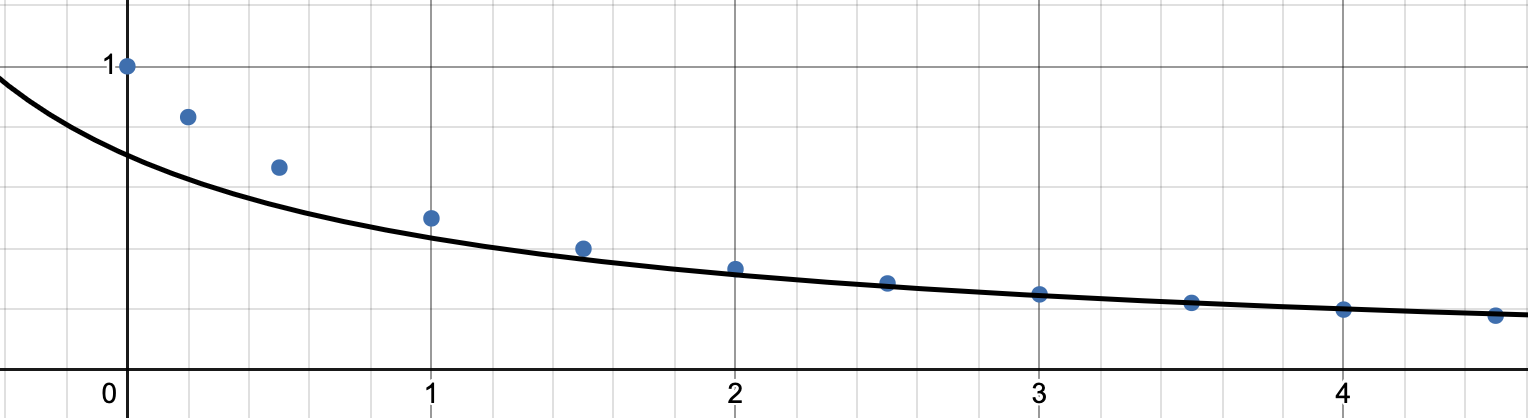
\includegraphics[width=.9\textwidth]{inv.png}\\
    График 1. Обратная модель
\end{center}

\section*{Решение при помощи дробной формулы}
Требуется сгладить при помощи формулы и вычислить невязки до тысячных.
\[ z = \frac{t}{a + bt} \]

Линеаризуем формулу:
\[z =\frac{t}{a+bt}\]
\[\frac{1}{z} = \frac{a+bt}{t} = \frac{a}{t} + b\]
\[z^{-1} = at^{-1}+b\]
\[y = z^{-1},\ x = t^{-1}\]
\begin{table}[H]
    \centering
    \begin{tabular}{|c|*{11}{c|}}
        \hline
        \(x\) & 5 & 2 & 1 & 0.667 & 0.5 & 0.4 & 0.333 & 0.286 & 0.25 & 0.222 \\
        \hline
        \(y\) & 1.2 & 1.5 & 2 & 2.5& 3.033 & 3.497 & 4 & 4.545 & 5 & 5.556 \\
        \hline
    \end{tabular}
\end{table}
На основе полученной таблицы найдём точечную оценку линейной модели.
\[
y = \tilde{b} + \tilde{a} x
\]
\textbf{Метод наименьших квадратов:}
\\ \\
\[S(a,\ b) = \sum_{i=1}^{n}(y_i - \tilde{y}(x_i))^2 = \sum_{i=1}^{10}(y_i - \tilde{b} - \tilde{a}x_i)^2\ ->\ min\]

Найдём экстремум:
\[\begin{cases}
    \pdv{S}{a} = -2\left(\sum_{i=1}^{10}y_i - 10\tilde{b} - \tilde{a}\sum_{i=1}^{10}x_i\right) = 0\\
    \pdv{S}{b} = -2\left(\sum_{i=1}^{10}x_iy_i - \tilde{b}\sum_{i=1}^{10}x_i - \tilde{a}\sum_{i=1}^{10}x_i^2\right) = 0
\end{cases}\]
\[\sum_{i=1}^{11}x_i = 10.658\]
\[\sum_{i=1}^{11}y_i = 32.826\]
\[\sum_{i=1}^{11}x_i^2 = 31.160\]
\[\sum_{i=1}^{11}x_iy_i = 20.697\]
\\
После подсчёта сумм получили систему:
\[\begin{cases}
    10\tilde{b} + 10.658\tilde{a} = 32.826\\
    10.658\tilde{b} + 31.160\tilde{a} = 20.697
\end{cases}\]
Подсчитали неизвестные:
\[\begin{cases}
    \tilde{b}  \approx 4.05\\
    \tilde{a}  \approx -0.72
\end{cases}\]
Подставили коэффиценты и получили точечную оценку:
\[\tilde{y} = 4.05 - 0.72x\]
В итоге получили точечную оценку
\[\tilde{z} = \frac{t}{-0.72 + 4.05t}\]
Вычисленные значения полученной оценки и невязки.
\begin{table}[H]
    \centering
    \begin{tabular}{|c|*{10}{c|}}
        \hline
        \(t\) & 0.2 & 0.5 & 1 & 1.5 & 2 & 2.5 & 3 & 3.5 & 4 & 4.5 \\
        \hline
        \(z\) &0.833&0.667 & 0.5& 0.4& 0.33& 0.286& 0.25& 0.22& 0.2& 0.18 \\
        \hline
        \(\tilde{z}\) & 2.222 & 0.383 & 0.300 & 0.280 & 0.271& 0.266& 0.262 & 0.260 & 0.258 & 0.257 \\
        \hline
        \(\epsilon\) & -1.389 & 0.284 & 0.200 & 0.120 & 0.059& 0.020 & -0.012 & -0.040 & -0.058 & -0.077  \\
        \hline
    \end{tabular}
\end{table}
\begin{center}
    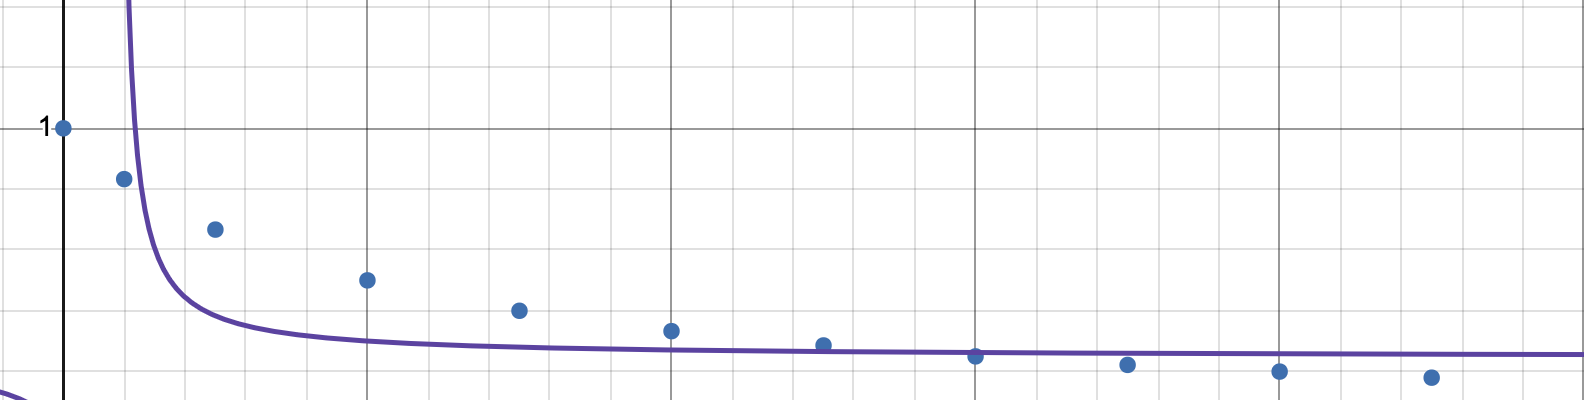
\includegraphics[width=.9\textwidth]{drob.png}\\
    График 2. Дробная модель
\end{center}

\section*{Решение при помощи степенной формулы}
Требуется сгладить при помощи формулы и вычислить невязки до тысячных.
\[ z = at^b \]

Линеаризуем формулу:
\[z = at^b\]
\[ln\ z = ln\ at^b = ln\ a+ln\ t^b = ln\ a +bln\ t\]
\[ln\ z = ln\ a+bln\ t\]
\[y = ln\ z,\ x = ln\ t, c = ln\ a\]
\begin{table}[H]
    \centering
    \begin{tabular}{|c|c|c|c|c|c|c|c|c|c|c|}
        \hline
        $x$ & $-1.609$&$-0.693$&$0 $& $0.405$ & $0.693$ & $0.916$ & $1.099$& $1.253$& $1.386$& $1.504$ \\
        \hline
        $y$ & $-0.182$ & $-0.405$ & $-0.693$ & $-0.916$ & $-1.109$ & $-1.252$& $-1.386$& $-1.514$& $-1.609$& $-1.715$ \\
        \hline
    \end{tabular}
\end{table}
На основе полученной таблицы найдём точечную оценку линейной модели.
\[
y = \tilde{c} + \tilde{b} x
\]
\textbf{Метод наименьших квадратов:}
\\ \\
\[S(a,\ b) = \sum_{i=1}^{n}(y_i - \tilde{y}(x_i))^2 = \sum_{i=1}^{10}(y_i - \tilde{c} - \tilde{b}x_i)^2\ ->\ min\]

Найдём экстремум:
\[\begin{cases}
    \pdv{S}{a} = -2\left(\sum_{i=1}^{10}y_i - 10\tilde{c} - \tilde{b}\sum_{i=1}^{10}x_i\right) = 0\\
    \pdv{S}{b} = -2\left(\sum_{i=1}^{10}x_iy_i - \tilde{c}\sum_{i=1}^{10}x_i - \tilde{b}\sum_{i=1}^{10}x_i^2\right) = 0
\end{cases}\]
\[\sum_{i=1}^{11}x_i = 4.954\]
\[\sum_{i=1}^{11}y_i = -10.781\]
\[\sum_{i=1}^{11}x_i^2 = 11.513\]
\[\sum_{i=1}^{11}x_iy_i = -9.943\]
\\
После подсчёта сумм получили систему:
\[\begin{cases}
    10\tilde{c} + 4.954\tilde{a} = -10.781\\
    4.954\tilde{b} + 11.513\tilde{a} = -9.943
\end{cases}\]
Подсчитали неизвестные:
\[\begin{cases}
    \tilde{b}  \approx -0.826\\
    \tilde{a}  \approx -0.508
\end{cases}\]
Подставили коэффиценты и получили точечную оценку:
\[\tilde{a} \approx 0.438\]
В итоге получили точечную оценку
\[\tilde{z} = 0.438t^{-0.508}\]
Вычисленные значения полученной оценки и невязки.
\begin{table}[H]
    \centering
    \begin{tabular}{|c|*{10}{c|}}
        \hline
        \(t\) & 0.2 & 0.5 & 1 & 1.5 & 2 & 2.5 & 3 & 3.5 & 4 & 4.5 \\
        \hline
        \(z\) &0.833&0.667 & 0.5& 0.4& 0.33& 0.286& 0.25& 0.22& 0.2& 0.18 \\
        \hline
        \(\tilde{z}\) & 0.992 & 0.623 & 0.438 & 0.356 & 0.308& 0.275& 0.251 & 0.232 & 0.217 & 0.204 \\
        \hline
        \(\epsilon\) & -0.159 & 0.044 & 0.062 & 0.044 & 0.022& 0.011 & -0.001 & -0.012 & -0.017 & -0.024  \\
        \hline
    \end{tabular}
\end{table}
\begin{center}
    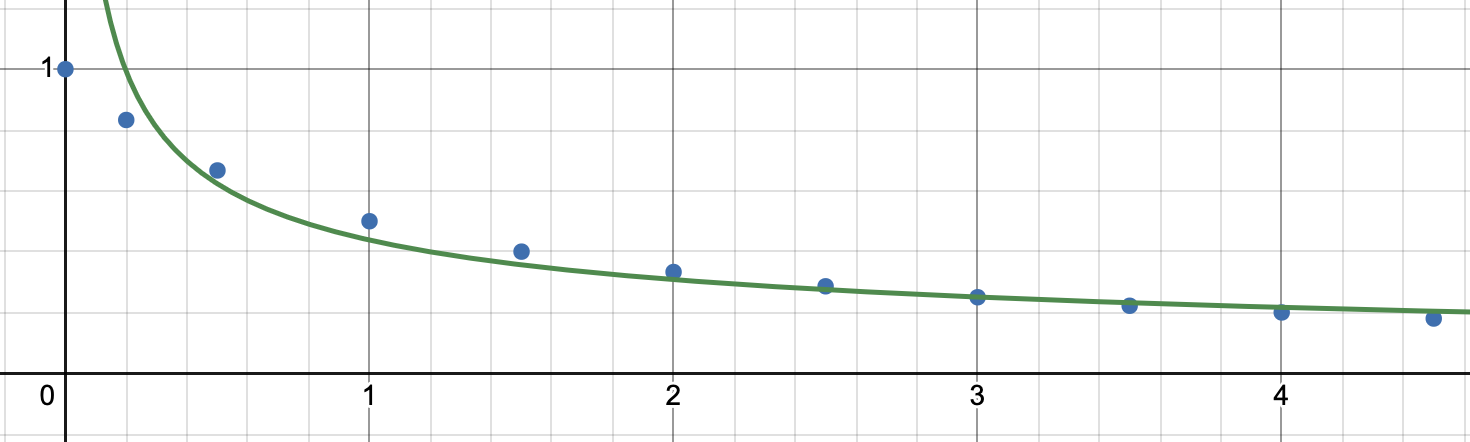
\includegraphics[width=.9\textwidth]{pow.png}\\
    График 3. Степенная модель
\end{center}

\section*{Решение при помощи экспоненциальной формулы}
Требуется сгладить при помощи формулы и вычислить невязки до тысячных.
\[ z = ae^{bt}\]

Линеаризуем формулу:
\[z = ae^{bt}\]
\[ln\ z = ln\ ae^b = ln\ a+ln\ e^{bt} - ln\ a + bt\]
\[ln\ z = ln\ a+bt\]
\[y = ln\ z;\ x=t;\ c = ln\ a\]
\begin{table}[H]
    \centering
    \begin{tabular}{|c|c|c|c|c|c|c|c|c|c|c|c|}
        \hline
        \(x\) & 0 & 0.2 & 0.5 & 1 & 1.5 & 2 & 2.5 & 3 & 3.5 & 4 & 4.5 \\
        \hline
        $y$ & 0& $-0.182$ & $-0.405$ & $-0.693$ & $-0.916$ & $-1.109$ & $-1.252$& $-1.386$& $-1.514$& $-1.609$& $-1.715$ \\
        \hline
    \end{tabular}
\end{table}
На основе полученной таблицы найдём точечную оценку линейной модели.
\[
y = \tilde{c} + \tilde{b} x
\]
\textbf{Метод наименьших квадратов:}
\\ \\
\[S(a,\ b) = \sum_{i=1}^{n}(y_i - \tilde{y}(x_i))^2 = \sum_{i=1}^{11}(y_i - \tilde{c} - \tilde{b}x_i)^2\ ->\ min\]

Найдём экстремум:
\[\begin{cases}
    \pdv{S}{a} = -2\left(\sum_{i=1}^{11}y_i - 11\tilde{c} - \tilde{b}\sum_{i=1}^{11}x_i\right) = 0\\
    \pdv{S}{b} = -2\left(\sum_{i=1}^{11}x_iy_i - \tilde{c}\sum_{i=1}^{11}x_i - \tilde{b}\sum_{i=1}^{11}x_i^2\right) = 0
\end{cases}\]
\[\sum_{i=1}^{11}x_i = 21.7\]
\[\sum_{i=1}^{11}y_i = -10.781\]
\[\sum_{i=1}^{11}x_i^2 = 69.29\]
\[\sum_{i=1}^{11}x_iy_i = -31.266\]
\\
После подсчёта сумм получили систему:
\[\begin{cases}
    11\tilde{c} + 21.7\tilde{a} = -10.781\\
    21.7\tilde{b} + 69.29\tilde{a} = -31.266
\end{cases}\]
Подсчитали неизвестные:
\[\begin{cases}
    \tilde{c}  \approx -0.307\\
    \tilde{b}  \approx -0.355
\end{cases}\]
Подставили коэффиценты и получили точечную оценку:
\[\tilde{a} \approx 0.734\]
В итоге получили точечную оценку
\[\tilde{z} = 0.734e^{-0.355t}\]
Вычисленные значения полученной оценки и невязки.
\begin{table}[H]
    \centering
    \begin{tabular}{|c|*{11}{c|}}
        \hline
        \(t\)&0 & 0.2 & 0.5 & 1 & 1.5 & 2 & 2.5 & 3 & 3.5 & 4 & 4.5 \\
        \hline
        \(z\)&1 &0.833&0.667 & 0.5& 0.4& 0.33& 0.286& 0.25& 0.22& 0.2& 0.18 \\
        \hline
        \(\tilde{z}\) & 0.734 & 0.684 & 0.615 & 0.515 & 0.431& 0.361& 0.302 & 0.253 & 0.212 & 0.177 & 0.149 \\
        \hline
        \(\epsilon\) & 0.266 & 0.149 & 0.052 & -0.015 & -0.031& -0.031 & -0.016 & -0.003 & 0.008 & 0.023& 0.031  \\
        \hline
    \end{tabular}
\end{table}
\begin{center}
    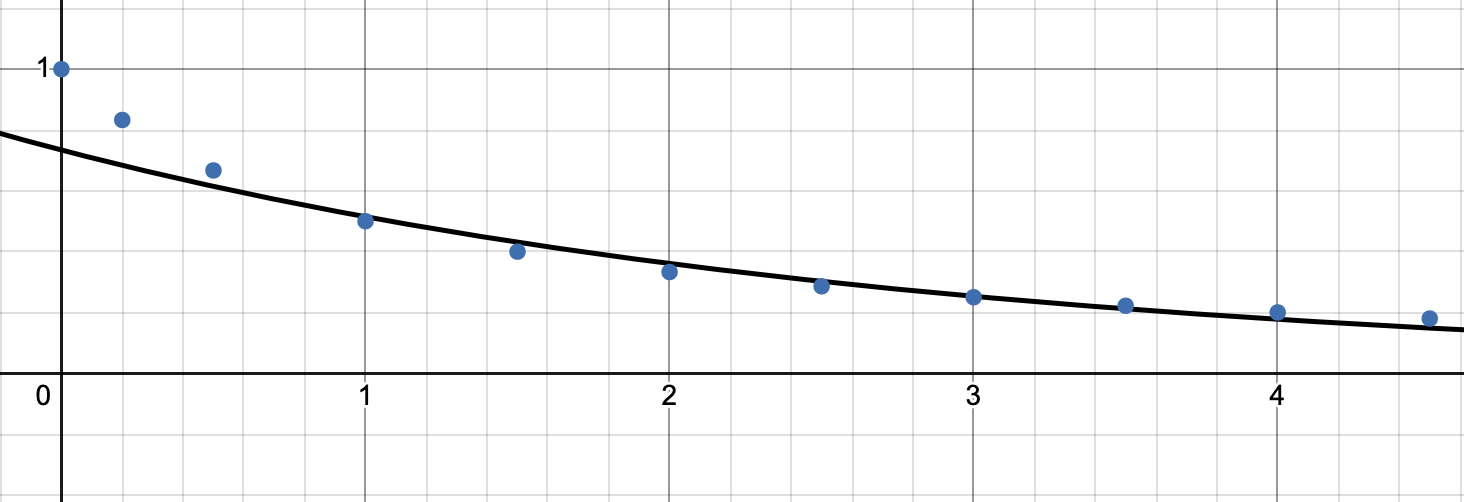
\includegraphics[width=.9\textwidth]{exp.png}\\
    График 4. Экспоненциальная модель
\end{center}

\section*{Вывод}

Используя метод наименьших квадратов, сгладили
предложенную табличную зависимость при помощи формул. 
Помимо этого, вычислили невязки с точностью до сотых и отобразить на графике табличные данные и сглаживающую кривую. 


\end{document}


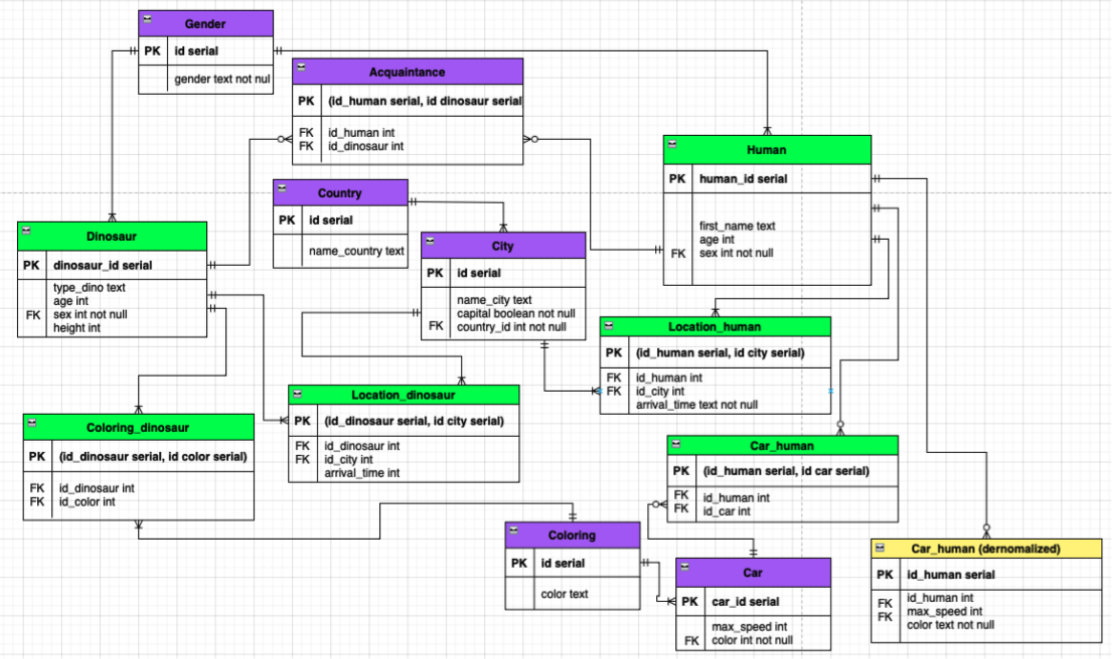
\includegraphics[width=.9\textwidth]{123}


